\subsection{Problem 5: Pelampung yang Berbohong}

\subsubsection{Identifikasi Masalah}

Sumber \texttt{SENSOR\_PANTAI} merupakan komponen yang paling kritis sekaligus paling tidak dapat dipercaya. Satu peringatan tsunami yang hilang dapat mengancam keselamatan warga pesisir, namun kode pengirim berasal dari luar kendali tim (\path{sustuna/sensor-pantai}). Kondisi tersebut memunculkan lima persoalan ketahanan utama dari arsitektur Milestone 1:

\begin{enumerate}
  \item \textbf{Hilangnya peringatan kritis atau keterlambatan melebihi 5 detik (Kriteria 1).}
  Saat terjadi lonjakan observasi atau gangguan pada \textit{broker} maupun basis data, pemrosesan berurutan halaman demi halaman dapat menunda peringatan \texttt{critical} melewati tenggat $p_{95} \le 5\text{ detik}$. Peringatan juga berisiko hilang saat kepemimpinan \textit{pod} berpindah. Dalam literatur, hal ini diselesaikan lewat \textbf{\textit{priority lane processing}} dan \textbf{\textit{transactional delivery ledger}} dengan pengiriman minimal sekali.

  \item \textbf{Data menyimpang dan pelanggaran kontrak yang mencemari koleksi kanonik (Kriteria 2).}
  Sensor dapat mengirim JSON cacat, kolom wajib kosong, nilai gelombang tidak masuk akal, waktu di masa depan terhadap \texttt{generated\_at}, atau memakai ulang \texttt{observation\_id} untuk isi kejadian berbeda. Membiarkan pesan tersebut tersimpan akan merusak kualitas data, sedangkan membuangnya menghapus jejak audit. Persoalan ini dikenal sebagai \textbf{\textit{data contract violation}} dan ditangani dengan pola \textbf{\textit{quarantine}}.

  \item \textbf{Rambatan latensi dari Sensor Pantai ke sumber lain (Kriteria 3).}
  Apabila seluruh sumber berbagi \textit{pool} koneksi dan \textit{loop} pengambilan yang sama tanpa pembatas konkurensi serta batas waktu tegas, sensor pantai yang lambat atau mengirim \textit{payload} raksasa akan menyita sumber daya. Akibatnya, pengambilan data BMKG, PVMBG, dan SATELIT ikut terhambat. Persoalan ini disebut \textbf{\textit{cascading failure}}, yang diisolasi dengan \textbf{\textit{bulkhead pattern}}, \textbf{\textit{bounded timeout}}, dan \textbf{\textit{capped streaming}}.

  \item \textbf{Badai percobaan ulang dan status sehat palsu dari sensor (Kriteria 4).}
  Memanggil ulang sensor yang bermasalah tanpa henti menciptakan \textbf{\textit{retry storm}} dan membuat klien menunggu hingga batas \textit{timeout}. Selain itu, \textit{endpoint} \path{/healthz} sensor dapat mengaku sehat meski jam \texttt{generated\_at} membeku atau datanya sudah usang berjam-jam. Kondisi ini membutuhkan \textbf{\textit{circuit breaker pattern}}, pemeriksaan kesegaran semantik, dan \textbf{\textit{fail-fast degradation}}.

  \item \textbf{Kelebihan beban yang mengorbankan lalu lintas Tim Lapangan (Kriteria 5).}
  Ketika banjir permintaan baca dari Media berbarengan dengan laporan Tim Lapangan, pembatasan rata-rata tanpa pembedaan kelas membuat kapasitas habis dimakan klien prioritas rendah. Dalam literatur, persoalan ini diselesaikan memakai \textbf{\textit{priority admission control}} dan \textbf{\textit{priority load shedding}}.
\end{enumerate}

\subsubsection{Rancangan Solusi dan Mekanisme yang Dipilih}

Solusi Problem 5 menerapkan pertahanan berlapis mulai dari klien pengambil data sensor, isolasi jalur antar-sumber, catatan pengiriman kritis, hingga gerbang \texttt{client-api} serta observabilitas menyeluruh. Rancangan lengkapnya diperlihatkan pada \textbf{Gambar~\ref{fig:p5-arch}}.

\begin{figure}[H]
  \centering
  \IfFileExists{figures/p5-arsitektur-ketahanan-pantai.png}{%
    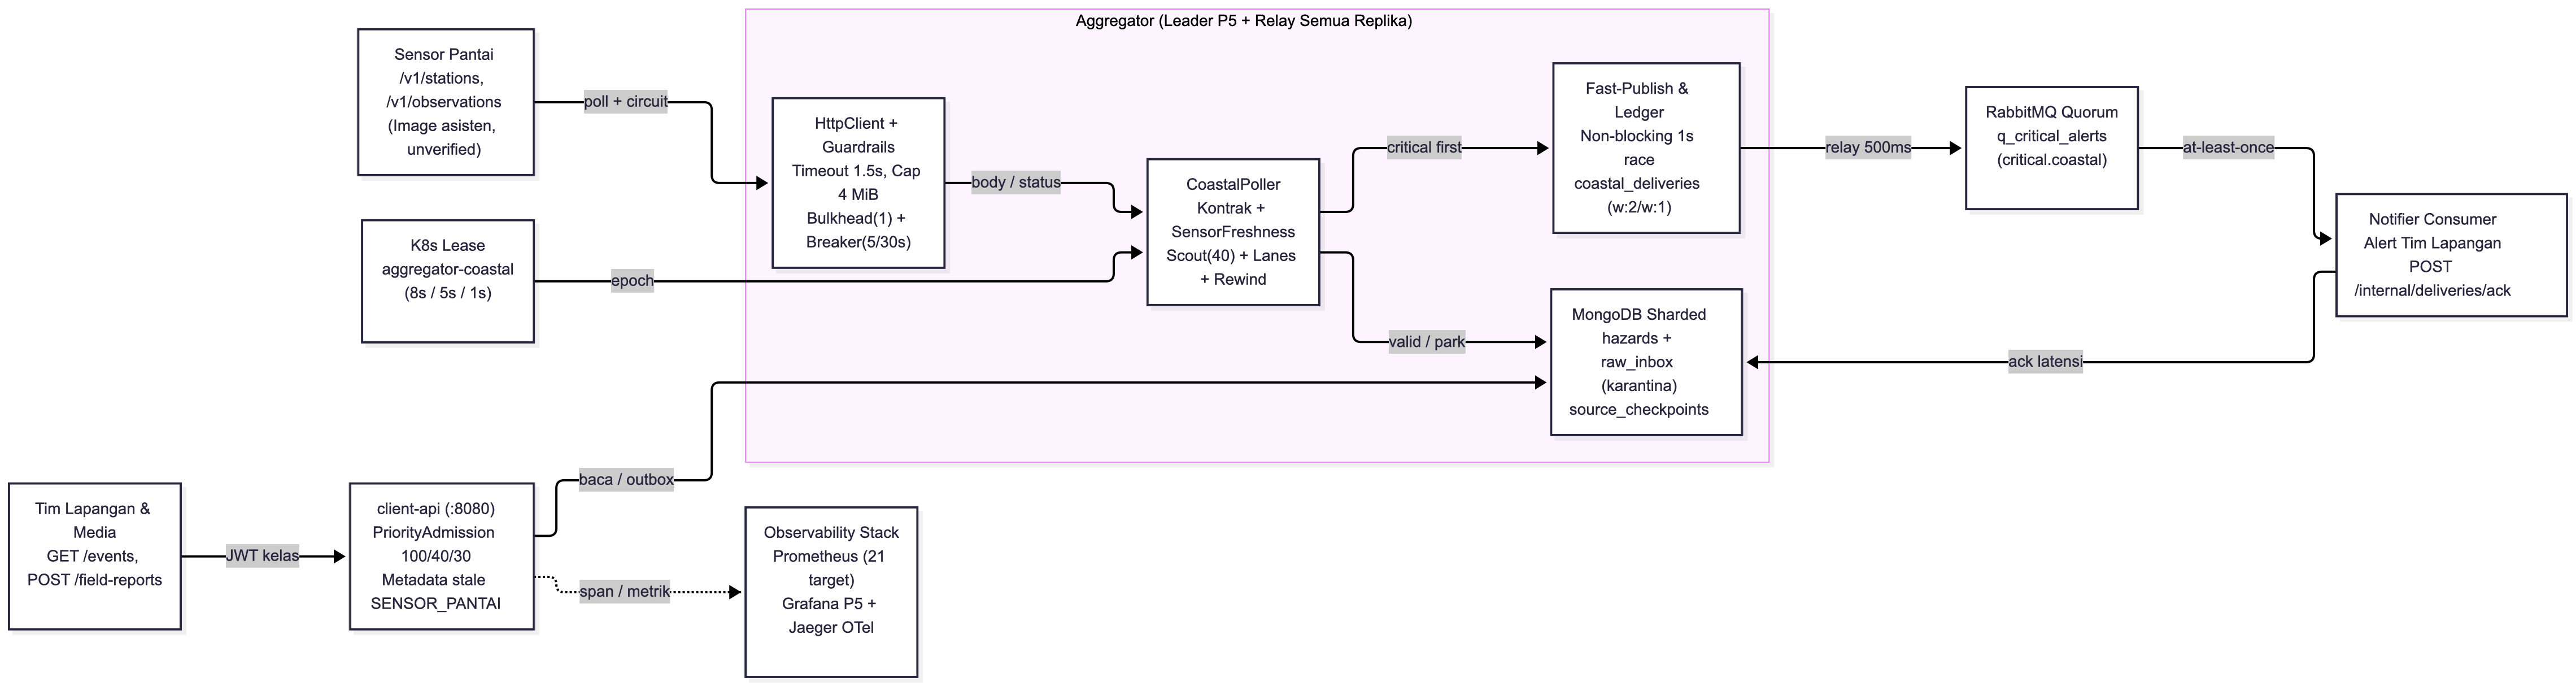
\includegraphics[width=0.95\linewidth]{p5-arsitektur-ketahanan-pantai.png}%
  }{%
  \resizebox{\linewidth}{!}{%
  \begin{tikzpicture}[
    every node/.style={font=\sffamily\footnotesize},
    box/.style={draw=black!65, rounded corners=3pt, fill=white, align=center, inner sep=5pt, minimum width=3.1cm, minimum height=0.92cm},
    crit/.style={draw=red!65!black, rounded corners=3pt, fill=red!6, align=center, inner sep=5pt, minimum width=3.1cm, minimum height=0.92cm},
    store/.style={draw=blue!55!black, rounded corners=2pt, fill=blue!6, align=center, inner sep=5pt, minimum width=3.2cm, minimum height=0.92cm},
    group/.style={draw=black!35, dashed, rounded corners=4pt, fill=black!2, inner sep=9pt},
    arr/.style={-{Stealth[length=2.2mm]}, thick, draw=black!75},
    lbl/.style={font=\sffamily\scriptsize, fill=white, inner sep=1.5pt, align=center}
  ]
    % Kiri: Sumber Eksternal & Klien
    \node[box]  (sensor) at (0, 4.4) {\textbf{Sensor Pantai}\\{\scriptsize /v1/stations, /v1/observations}\\{\scriptsize (Image asisten, unverified)}};
    \node[box]  (lease)  at (0, 2.2) {\textbf{K8s Lease}\\{\scriptsize aggregator-coastal}\\{\scriptsize ($8\text{s} / 5\text{s} / 1\text{s}$)}};
    \node[box]  (cli)    at (0, 0.0) {\textbf{Tim Lapangan \& Media}\\{\scriptsize GET /events, POST /field-reports}};

    % Kolom 2: Guardrails & Gateway
    \node[box]  (guard)  at (6.2, 4.4) {\textbf{HttpClient + Guardrails}\\{\scriptsize Timeout $1{,}5\text{s}$, Cap $4\text{ MiB}$}\\{\scriptsize Bulkhead(1) + Breaker($5/30\text{s}$)}};
    \node[box]  (poller) at (6.2, 2.2) {\textbf{CoastalPoller}\\{\scriptsize Kontrak + SensorFreshness}\\{\scriptsize Scout($40$) + Lanes + Rewind}};
    \node[box]  (capi)   at (6.2, 0.0) {\textbf{client-api (:8080)}\\{\scriptsize PriorityAdmission $100/40/30$}\\{\scriptsize Metadata stale SENSOR\_PANTAI}};

    % Kolom 3: Delivery & Store
    \node[crit]  (fast)  at (12.8, 4.4) {\textbf{Fast-Publish \& Ledger}\\{\scriptsize Non-blocking $1\text{s}$ race}\\{\scriptsize coastal\_deliveries ($w:2/w:1$)}};
    \node[store] (mongo) at (12.8, 2.2) {\textbf{MongoDB Sharded}\\{\scriptsize hazards + raw\_inbox (karantina)}\\{\scriptsize source\_checkpoints}};
    \node[box]   (obs)   at (12.8, 0.0) {\textbf{Observability Stack}\\{\scriptsize Prometheus (21 target)}\\{\scriptsize Grafana P5 + Jaeger OTel}};

    % Kolom 4: Broker & Notifier
    \node[crit] (rmq)  at (19.0, 4.4) {\textbf{RabbitMQ Quorum}\\{\scriptsize q\_critical\_alerts}\\{\scriptsize (critical.coastal)}};
    \node[crit] (noti) at (19.0, 2.2) {\textbf{Notifier Consumer}\\{\scriptsize Alert Tim Lapangan}\\{\scriptsize POST /internal/deliveries/ack}};

    % Grouping
    \begin{scope}[on background layer]
      \node[group, fit=(guard)(poller)(fast)(mongo), label={[font=\sffamily\scriptsize\bfseries]above:Aggregator (Leader P5 + Relay Semua Replika)}] {};
    \end{scope}

    % Panah
    \draw[arr] (sensor) -- node[lbl, above] {poll + circuit} (guard);
    \draw[arr] (lease)  -- node[lbl, above] {epoch} (poller);
    \draw[arr] (guard)  -- node[lbl, left] {body/status} (poller);
    \draw[arr] (poller.north east) -- node[lbl, above, sloped] {critical first} (fast.south west);
    \draw[arr] (poller) -- node[lbl, above] {valid / park} (mongo);
    \draw[arr] (fast)   -- node[lbl, above] {relay $500\text{ms}$} (rmq);
    \draw[arr] (rmq)    -- node[lbl, left] {at-least-once} (noti);
    \draw[arr] (noti.south west) -- node[lbl, above, sloped] {ack latensi} (mongo.south east);

    \draw[arr] (cli) -- node[lbl, above] {JWT kelas} (capi);
    \draw[arr] (capi) -- node[lbl, above] {baca / outbox} (mongo);
    \draw[arr, dashed] (capi) -- node[lbl, above] {span/metrik} (obs);
  \end{tikzpicture}%
  }%
  }
  \caption{Diagram Rancangan Arsitektur Ketahanan dan Prioritas pada Problem 5}
  \label{fig:p5-arch}
\end{figure}

Secara terperinci, ketahanan Problem 5 bertumpu pada lima mekanisme utama berikut.

\paragraph*{1. Validasi Kontrak Ketat, Penanganan Konflik ID, dan Karantina}
Sebelum data menyentuh koleksi kanonik, \texttt{refreshStations} memvalidasi daftar stasiun dari \path{/v1/stations} (\path{aggregator/src/coastal/contract.ts}). Fungsi \texttt{validateObservation} lalu memeriksa tujuh kolom wajib, tipe data, format UTC, keberadaan stasiun, serta kewajaran fisis ($|\text{anomali muka laut}| \le 30\text{ m}$ dan $0 \le \text{tinggi gelombang} \le 40\text{ m}$).

Setiap item yang melanggar langsung dikarantina ke \path{raw_inbox} disertai alasan eksplisit. Bila item cacat bertanda \texttt{critical}, sistem menaikkan metrik \path{coastal_quarantined_critical_total} dan mencatat log \texttt{error}. Jika sensor memakai ulang \texttt{observation\_id} dengan isi berbeda (\texttt{contentSignature}), fungsi \texttt{variantRef} memberi akhiran hash unik agar peristiwa baru tidak tertelan duplikasi palsu.

\paragraph*{2. Isolasi Sumber melalui \textit{Bulkhead}, \textit{Timeout}, \textit{Circuit Breaker}, dan \textit{SensorFreshness}}
Empat pengaman menjaga agar kerusakan Sensor Pantai tidak menjalar ke komponen lain:

\begin{itemize}
  \item \textbf{\texttt{HttpSensorClient} (\path{sensorClient.ts}):} memakai batas waktu tunggal \path{1.500 ms} mencakup fase koneksi hingga isi respons serta batas \textit{stream} \path{4 MiB} (\texttt{readCapped}) agar \textit{payload} besar tidak menguras memori.
  \item \textbf{\texttt{Bulkhead('coastal', 1)} (\path{bulkhead.ts}):} membatasi maksimal satu siklus \textit{polling} pantai yang aktif bersamaan dan memisahkannya dari \textit{loop} serta \textit{lease} BMKG, PVMBG, dan SATELIT.
  \item \textbf{\texttt{CircuitBreaker} (\path{breaker.ts}):} membuka sirkuit setelah \texttt{5} kegagalan dalam \texttt{30.000 ms}, menahan permintaan $2.000$--$5.000\text{ ms}$ dengan acakan \textit{jitter} $\pm 20\%$, lalu mengirim satu uji pemulihan pada status \textit{half-open}.
  \item \textbf{\texttt{SensorFreshness} (\path{freshness.ts}):} mengabaikan \path{/healthz} dan memantau jam internal sensor. Status menjadi \texttt{frozen\_clock} jika \texttt{generated\_at} berhenti $\ge 5\text{ detik}$, serta \texttt{stale} jika \textit{lag} di akhir log melebihi \texttt{120 detik}. Keduanya memicu \textit{breaker} sekaligus menandai \texttt{stale: true} pada \path{/events}.
\end{itemize}

\paragraph*{3. Jalur Cepat Peringatan Kritis dan \textit{Delivery Ledger}}
Saat halaman penuh terdeteksi (\texttt{500} item), fungsi \texttt{scout()} menengok hingga \texttt{40} halaman ke depan untuk mengambil lebih dahulu seluruh peristiwa \texttt{critical: true}. Di halaman aktif, jalur \texttt{critical} juga diproses sebelum observasi biasa (\path{poller.ts}).

Pengiriman kritis memakai jalur ganda. Pertama, \texttt{fastPublish} mengirim paralel non-blocking ke antrean \textit{quorum} \path{q_critical_alerts} dengan batas tunggu \texttt{1.000 ms}. Kedua, \texttt{MongoDeliveryLedger} (\path{ledger.ts}) mencatat pengiriman di \path{coastal_deliveries} memakai \textit{write concern} adaptif \texttt{bookkeepingOptions()} ($w:2$ saat normal, $w:1$ saat terdegradasi). Seluruh replika lalu menyalurkan ulang antrean tiap \texttt{500 ms} hingga \texttt{notifier} memanggil \path{POST /internal/deliveries/ack}.

\paragraph*{4. Partisi Kapasitas dan \textit{Priority Load Shedding}}
Setelah autentikasi JWT menentukan kelas klien (\texttt{field-team}, \texttt{bnpb-ops}, atau \texttt{media}), \textit{middleware} \texttt{priorityAdmission} membagi kapasitas tanpa antrean di \path{client-api/src/middleware/admission.ts}. Nilai baku memakai \path{MAX_IN_FLIGHT = 100}, \path{RESERVED_FIELD_TEAM = 40}, dan \path{MEDIA_MAX_IN_FLIGHT = 30}.

Dengan rumus partisi ini, gabungan \texttt{ops + media} maksimal hanya memakai $60$ slot dan \texttt{media} dibatasi maksimal $30$ slot. Sebanyak $40$ slot eksklusif selalu tersisa untuk \texttt{field-team}, sedangkan kelebihan beban langsung ditolak cepat dengan HTTP \texttt{429 Retry-After: 1}.

\paragraph*{5. Observabilitas dan Penetapan SLO beserta \textit{Error Budget}}
Sistem mengekspor metrik Prometheus dari 21 target \textit{pod} ke Grafana (dasbor 12 panel untuk ketahanan pantai), log JSON Pino ber-\texttt{correlation\_id}, serta jejak \textit{tracing} OpenTelemetry ke Jaeger (\path{docs/m2/observability.md}). Dua target keandalan ditetapkan pada \path{docs/m2/slo.md}: \textbf{99\% ketepatan waktu} pengiriman kritis dalam $\le 5\text{ detik}$ (\textit{error budget} $1\%$) serta \textbf{99,5\% admitansi} permintaan Tim Lapangan di \texttt{client-api} (\textit{error budget} $0{,}5\%$).

\subsubsection{Alasan Keputusan}

\textbf{Tabel~\ref{tab:p5-decisions}} merangkum keputusan desain utama Problem 5, alasan dan konsekuensinya, serta alternatif yang ditolak.

\begin{small}
\begin{longtable}{@{} >{\raggedright\arraybackslash}p{3.4cm} >{\raggedright\arraybackslash}p{7.4cm} >{\raggedright\arraybackslash}p{4.0cm} @{}}
  \caption{Desain, Alasan, dan Alternatif yang Ditolak pada Problem 5}
  \label{tab:p5-decisions} \\
  \toprule
  \textbf{Keputusan} & \textbf{Alasan} & \textbf{Alternatif (Ditolak)} \\
  \midrule
  \endfirsthead
  \caption[]{Desain, Alasan, dan Alternatif yang Ditolak pada Problem 5 (Lanjutan)} \\
  \toprule
  \textbf{Keputusan} & \textbf{Alasan} & \textbf{Alternatif (Ditolak)} \\
  \midrule
  \endhead
  \midrule
  \multicolumn{3}{r}{\textit{Bersambung ke halaman berikutnya...}} \\
  \endfoot
  \bottomrule
  \endlastfoot
  \textit{Circuit Breaker} ($5$ gagal/$30\text{s}$, open $2$--$5\text{s}$) bersama \texttt{Sensor\-Freshness} & Memutus panggilan begitu \textit{error} beruntun maupun ketika sensor berbohong dengan jam beku atau data usang melebihi $120\text{ s}$. Uji pemulihan tetap berjalan otomatis tiap $2$--$5\text{ detik}$. Konsekuensinya, jeda deteksi pulih berkisar $2$--$6\text{ detik}$. & \textbf{Mengandalkan \path{/healthz} atau buka sirkuit terlalu lama:} gagal mendeteksi kepalsuan data dan memperlambat pemulihan otomatis saat sensor sudah sembuh. \\
  \midrule
  \texttt{Bulkhead} (\texttt{coastal=1}) + \textit{timeout} tunggal $1.500\text{ ms}$ + batas $4\text{ MiB}$ & Mengurung penggunaan soket serta memori poller pantai pada satu slot aktif tanpa \textit{retry} berlapis. Sumber BMKG, PVMBG, dan SATELIT pun tetap cepat saat sensor pantai menggantung. Konsekuensinya, kegagalan diulang pada siklus berikutnya. & \textbf{\textit{Auto-retry} di klien HTTP plus \textit{pool} bersama:} memperpanjang pemblokiran hingga kelipatan \textit{timeout} dan menyumbat \textit{event loop} global. \\
  \midrule
  Jalur ganda: \texttt{fastPublish} non-blocking + \textit{delivery ledger} + \texttt{scout(40)} & Memisahkan peringatan mendesak dari antrean biasa. Fungsi \texttt{scout(40)} menarik data kritis dari tengah antrean, \texttt{fastPublish} mengirim cepat ke \textit{broker}, dan \textit{ledger} di seluruh \textit{pod} menjamin nol kehilangan saat pemimpin berganti. & \textbf{Menulis sinkron sekuensial halaman per halaman:} lonjakan observasi biasa atau satu \textit{node} lambat langsung membuat peringatan kritis lewat $5\text{ detik}$. \\
  \midrule
  \texttt{Priority\-Admission} partisi statis ($100/40/30$) di \texttt{client-api} & Menjamin 40 slot khusus untuk \texttt{field-team} yang mustahil diserobot \texttt{media} (batas 30). Kelebihan beban ditolak seketika dengan \texttt{429} agar memori \texttt{256Mi} aman. Konsekuensinya, \texttt{media} tetap terbatasi di 30 meski lalu lintas sepi. & \textbf{Antrean prioritas di RAM atau batas per-IP rata:} antrean memperburuk \textit{tail latency} saat memori penuh, sedangkan batas rata meloloskan serbuan Media. \\
  \midrule
  Deteksi penyimpangan via \texttt{variantRef} dan \texttt{rewind} & Bila jam \texttt{generated\_at} mundur atau halaman kosong berkepanjangan saat sensor \textit{restart}, poller memutar ulang dari awal secara \textit{idempotent}. Jika ID lama berisi data baru, \texttt{variantRef} memisahkannya. Konsekuensinya, \textit{cache} \texttt{signatures} menyimpan hingga 20.000 entri. & \textbf{Menolak ID ganda atau menimpa diam-diam:} cara pertama berisiko membuang peringatan baru yang sah, sedangkan cara kedua menghapus bukti kejadian lama. \\
\end{longtable}
\end{small}

\subsubsection{Batasan yang Disadari}

\textbf{Tabel~\ref{tab:p5-limits}} mencatat batasan yang disadari pada modul pantai dan ketahanan sistem.

\begin{table}[H]
  \centering
  \caption{Batasan Implementasi yang Disadari pada Problem 5}
  \label{tab:p5-limits}
  \small
  \begin{tabularx}{\linewidth}{@{} >{\raggedright\arraybackslash}p{3.6cm} >{\raggedright\arraybackslash}X >{\raggedright\arraybackslash}p{4.1cm} @{}}
    \toprule
    \textbf{Batasan} & \textbf{Penjelasan dan Alasan} & \textbf{Referensi Kode} \\
    \midrule
    \textbf{\textit{Span} OpenTelemetry berhenti pada layanan pihak ketiga} & \textit{Mock}, MongoDB, RabbitMQ, dan \path{sensor-pantai} tidak memancarkan \textit{span} ke Jaeger. Pelacakan lintas \textit{broker} tetap tersambung lewat \texttt{correlation\_id} log dan \textit{field} \texttt{traceparent} di \path{coastal_deliveries}. & \path{docs/m2/observability.md}, \path{aggregator/src/coastal/ledger.ts} \\
    \midrule
    \textbf{Pengujian mati \textit{node} pada satu komputer fisik ($30$--$38\text{ s}$)} & Pada pengujian \texttt{node-loss}, mematikan satu VM berarti mematikan sebagian CPU dan memori komputer yang sama, dan k3s memerlukan sekitar $16\text{ detik}$ untuk menandai \textit{node} tak sehat. Akibatnya jeda serah terima \textit{leader} lebih lama ($p_{95} = 34\text{ s}$) daripada pada \textit{node} fisik terpisah. Seluruh 300/300 peringatan tetap sampai (0 hilang); yang terpengaruh hanya ambang 5 detik pada 196 peringatan yang dipancarkan saat serah terima. Pada kegagalan proses \textit{leader} p95 4,4 detik. & \path{aggregator/src/coastal/service.ts}, \path{docs/m2/slo.md}, \path{docs/m2/evidence/pc-run-phase2.md} \\
    \midrule
    \textbf{Kapasitas CPU komputer pengujian saat banjir Media} & \texttt{PriorityAdmission} mencatat 0 penolakan \texttt{429} untuk Tim Lapangan. Karena ketiga VM VirtualBox berbagi CPU satu komputer, banjir Media menaikkan $p_{95}$ baca menjadi $1{,}83$--$1{,}88\text{ s}$ serta memicu sedikit \textit{timeout} \texttt{2.000 ms} pada \path{POST /field-reports} walau laporan tetap tersimpan di \textit{outbox}. & \path{client-api/src/middleware/admission.ts}, \path{docs/m2/deviations.md} \\
    \midrule
    \textbf{Uji gabungan \textit{Tester Agent} (\textit{game day}) belum penuh} & Baru skenario \texttt{schema} yang lolos dari enam skenario latihan karena seluruh \textit{node} klaster k3s berperan sebagai \textit{control-plane}. Skenario ujian penuh juga menunggu kunci resmi saat demo. & \path{docs/m2/deviations.md}, \path{docs/m2/evidence/pc-run-phase2.md} \\
    \midrule
    \textbf{Keterbatasan perangkat keras pengujian} & Ketiga VM berbagi CPU satu komputer fisik yang hanya melayani sekitar 45 hingga 50 permintaan per detik untuk beban kerja M1 tanpa jeda berpikir, sehingga bukti memakai skala beban yang disesuaikan dengan kapasitas komputer ini: empat pengguna M1 dan batas Media 4 permintaan bersamaan per \textit{pod} (baku 30). Ini batas \textit{host}, bukan batas rancangan prioritas. & \path{scripts/m2/p5-m1-load.sh}, \path{load-test/p5-priority.js} \\
    \bottomrule
  \end{tabularx}
\end{table}

\subsubsection{Bukti Penyelesaian per Kriteria}

Bukti berikut berasal dari eksekusi skrip pada klaster tiga VM (\texttt{node-a}, \texttt{node-c}, \texttt{node-d}). Keluaran teks lengkap tiap eksekusi tersimpan di repositori pada \path{docs/m2/proofs/}. Kegagalan disuntikkan melalui sensor palsu (\texttt{sensor-fake}) yang hanya dipakai saat pengujian; skenario \textit{game day} Tester Agent menunggu bahan pengujian dari asisten.


\paragraph*{Kriteria 1: 0 \textit{event} kritis hilang, $p_{95} \le 5$ detik.}
Pada kondisi normal 300 dari 300 \textit{alert} sampai ke penerima Tim Lapangan, p95 1.737 ms (p50 877 ms), dan tidak ada yang melewati 5 detik. Saat proses \textit{leader} pesisir dimatikan paksa, 400 dari 400 tetap terkirim dengan p95 4.447 ms; 16 \textit{alert} yang dipancarkan saat serah terima \textit{leader} melewati 5 detik secara individual. Pada uji terpisah, pemadaman \textit{node leader} pesisir sungguhan tidak menghilangkan \textit{alert}, tetapi jeda serah terima 30 hingga 38 detik membuat p95 sekitar 34 detik; hal ini dipengaruhi oleh keterbatasan pengujian pada satu komputer: ketiga VM berbagi CPU yang sama dengan VM yang dimatikan, sehingga pemulihan \textit{lease} lebih lambat daripada pada \textit{node} fisik terpisah (lihat bagian batasan).
\gambarbukti{bk-5-1a.png}{Pengiriman \textit{alert} kritis kondisi normal (\texttt{p5-latency.sh})}{bk-5-1a}
\gambarbukti{bk-5-1b.png}{Pengiriman \textit{alert} kritis saat proses \textit{leader} dimatikan paksa}{bk-5-1b}

\paragraph*{Kriteria 2: penyisihan data yang melanggar kontrak.}
Lima item yang melanggar kontrak dasar disuntikkan ke sensor palsu. Seluruhnya muncul dalam daftar pesan gagal Internal Ops dengan alasan (\texttt{missing\_field:observed\_at}, \texttt{out\_of\_range:wave\_height\_m}, \texttt{missing\_field:critical}), dan jumlah \texttt{HazardEvent} Sensor Pantai tidak berubah.
\gambarbukti{bk-5-2.png}{Data melanggar kontrak disisihkan beserta alasannya (\texttt{p5-quarantine.sh})}{bk-5-2}

\paragraph*{Kriteria 3: latensi sumber lain tetap terjaga.}
Beban kerja M1 (\path{load-test/events.js}) dijalankan pada empat pengguna (skala disesuaikan dengan kapasitas komputer pengujian yang melayani sekitar 45 hingga 50 permintaan per detik tanpa jeda berpikir): p95 SEISMIC 169 ms (sensor normal), 155 ms (lambat), dan 133 ms (tidak menjawab), semuanya di bawah 300 ms dan tanpa permintaan gagal. Sensor sakit tidak membuat sumber lain lebih lambat. Pada enam pengguna p95 berada di tepi batas (235 hingga 321 ms) dan pada 50 pengguna M1 asli p95 melampaui 300 ms walau sensor sehat karena kapasitas CPU komputer pengujian, bukan karena sensor sakit.
\gambarbukti{bk-5-3.png}{Latensi beban kerja M1 pada sensor normal, lambat, dan tidak menjawab (\texttt{p5-m1-load.sh})}{bk-5-3}

\paragraph*{Kriteria 4: \textit{circuit breaker} dan pemulihan otomatis.}
Pada enam mode sensor sakit (lambat, tidak menjawab, HTTP 503, rusak, basi, beku), permintaan ke sensor hanya 7 hingga 12 per 40 detik (dasar 38, batas 60), permintaan klien yang bergantung pada sensor dijawab dalam 44 hingga 59 ms dengan status 200, dan sistem memakai sensor lagi sendiri 1 hingga 4 detik setelah sensor pulih. Sumber lain tetap dengan p95 SEISMIC 47 hingga 80 ms. Seluruh 25 pemeriksaan lulus.
\gambarbukti{bk-5-4.png}{Enam mode Sensor Pantai sakit (\texttt{p5-checks.sh})}{bk-5-4}

\paragraph*{Kriteria 5: \textit{priority load shedding}.}
Dengan 40 pengguna Media dan 5 pengguna Tim Lapangan, batas Media diturunkan sementara menjadi 4 permintaan bersamaan per \textit{pod} (normalnya 30) menyesuaikan kapasitas komputer pengujian yang hanya melayani sekitar 50 permintaan per detik. Media ditolak terkontrol 16.889 kali (HTTP 429), Tim Lapangan dilayani penuh (452 pembacaan, 0 ditolak) dan seluruh 120 laporan diterima, dengan p95 981 ms (di bawah target internal 1 detik). Pada pengaturan baku dengan 100 pengguna Media, p95 Tim Lapangan sekitar 1,9 detik, yang mencerminkan kapasitas CPU komputer pengujian, bukan rancangan pembatas prioritas.
\gambarbukti{bk-5-5.png}{Media ditolak terkontrol sementara Tim Lapangan dilayani (\texttt{load-test/p5-priority.js})}{bk-5-5}

\paragraph*{Kriteria 6: \textit{game day} kombinasi kegagalan tanpa intervensi.}
\isian{Tambahkan log dan metrik pemulihan mandiri dari \textit{game day} Tester Agent setelah kunci skenario ujian dibagikan asisten.}

\paragraph*{Kriteria 7: diagnosis lewat dasbor, metrik, dan \textit{trace}.}
Satu laporan lapangan dilacak melalui seluruh \textit{hop}: \textit{client API}, \texttt{aggregator}, penulisan ke penyimpanan, publikasi ke \textit{broker}, tiga \textit{consumer}, dan \textit{acknowledgement} (9 \textit{span}, 237 ms) dengan \textit{correlation ID} yang sama pada tiap \textit{span}. Satu \textit{alert} pesisir dilacak dari \textit{polling} sensor, \textit{ingest}, \textit{relay}, \textit{consumer}, hingga \textit{acknowledgement} (20 \textit{span}). Dasbor koordinasi (\textit{leader} dan \textit{epoch}) serta dasbor pesisir melengkapi diagnosis.
\gambarbukti[0.30]{bk-5-7a.png}{Jejak satu laporan lapangan melalui seluruh \textit{hop}}{bk-5-7a}
\gambarbukti[0.40]{bk-5-7b.png}{Rincian \textit{trace} di Jaeger dengan \textit{correlation ID}}{bk-5-7b}
\gambarbukti[0.30]{bk-5-7c.png}{Jejak satu \textit{alert} kritis pesisir}{bk-5-7c}
\gambarbukti[0.40]{bk-5-7d.png}{Dasbor koordinasi: \textit{leader} dan \textit{epoch}, poll, dan penyimpanan}{bk-5-7d}
\gambarbukti[0.40]{bk-5-7e.png}{Dasbor ketahanan pesisir (\textit{circuit breaker} dan permintaan ke sensor)}{bk-5-7e}

\paragraph*{Kriteria 8: target keandalan dan \textit{error budget}.}
Target keandalan jalur peringatan Tim Lapangan didefinisikan pada \path{docs/m2/slo.md}. \isian{Tambahkan pemakaian \textit{error budget} selama \textit{game day} setelah skenario ujian dijalankan.}

\subsubsection{Jawaban atas Butir ``Di laporan''}

\paragraph*{Persoalan Ketahanan pada Kriteria 2--5 serta Arsitektur Konfigurasinya}
Kriteria 2 hingga 5 mencerminkan empat persoalan ketahanan klasik. Kriteria 2 menghadapi \textbf{\textit{data contract violation}} dan \textit{poison input} yang diatasi melalui validasi fisis serta pola \textbf{\textit{quarantine}}. Kriteria 3 menghadapi \textbf{\textit{cascading failure}} lintas sumber yang dicegah oleh \textbf{\textit{bulkhead pattern}} dan \textit{timeout} tunggal.

Pada Kriteria 4, pemanggilan ulang ke sensor bermasalah memicu \textbf{\textit{retry storm}} dan terkelabui oleh \textbf{\textit{liveness lie}} pada \path{/healthz}, yang ditangani memakai \textbf{\textit{circuit breaker}} serta pemeriksaan kesegaran semantik. Sementara itu, Kriteria 5 menyelesaikan \textbf{\textit{priority inversion under overload}} lewat \textbf{\textit{priority admission control}}.

Setiap ambang batas dirancang berdasarkan anggaran latensi $5\text{ detik}$ jalur peringatan kritis. \texttt{HttpSensorClient} memutus tunggu pada \texttt{1.500 ms} dan \texttt{4 MiB} agar panggilan gagal tidak menguras waktu. \texttt{Bulkhead('coastal', 1)} bersama interval \textit{polling} \texttt{1.000 ms} memastikan pengambilan pantai terkurung pada satu eksekusi aktif saja.

Sementara itu, \texttt{CircuitBreaker} membuka sirkuit setelah \texttt{5} kegagalan dalam \texttt{30.000 ms} untuk mengabaikan gangguan sesaat, lalu menutup akses selama $2$--$5\text{ detik}$ sebelum menguji pulih otomatis. \texttt{SensorFreshness} membandingkan \texttt{generated\_at} ($\ge 5\text{ s}$ beku) dan keterlambatan observasi ($> 120\text{ s}$) memakai jam internal sensor agar kebal terhadap \textit{clock skew}. Di gerbang masuk, \texttt{PriorityAdmission} mematok partisi \texttt{100/40/30} guna menjamin $40\%$ kapasitas eksklusif Tim Lapangan serta membatasi Media di $30\%$.

\paragraph*{Perilaku Menyimpang Sensor Pantai: Cara Menemukan dan Menanganinya}
Pengamatan terhadap kontrak dan pengujian enam mode gangguan (\path{p5-checks.sh}) mengungkap lima penyimpangan utama Sensor Pantai:

\begin{enumerate}
  \item \textbf{Status \path{/healthz} sehat palsu saat data membeku atau usang:} dideteksi oleh \texttt{SensorFreshness.evaluate} lewat kemandekan \texttt{generated\_at} ($\ge 5\text{ s}$) maupun \textit{lag} observasi ($> 120\text{ s}$). Sistem memicunya sebagai kegagalan \textit{breaker} dan menyertakan penanda \texttt{stale: true} di \path{/events}.
  \item \textbf{Jam sensor melompat mundur ($> 60\text{ s}$) atau kursor menggantung:} terpantau oleh \texttt{lastGeneratedMs} dan \texttt{blindCheck()} saat menerima halaman kosong melebihi $120\text{ s}$ waktu sensor. Sistem memanggil \texttt{rewind()} untuk mengulang pembacaan dari awal secara \textit{idempotent}.
  \item \textbf{Penggunaan ulang \texttt{observation\_id} dengan muatan berbeda:} dideteksi lewat perbandingan \texttt{contentSignature()} terhadap \textit{cache} \texttt{signatures} dan basis data. Fungsi \texttt{variantRef()} lalu membangkitkan akhiran hash unik agar data baru tidak tertimpa.
  \item \textbf{Pelanggaran skema, nilai fisis mustahil, atau stasiun senyap ($> 300\text{ s}$):} disaring oleh \texttt{validateObservation} lalu dikarantina ke \path{raw_inbox}. Stasiun asing memicu pembaruan stasiun berjeda $10\text{ detik}$, sementara pesan kritis cacat menyalakan metrik \textit{error} khusus operator.
  \item \textbf{Respons lambat, \textit{blackhole}, galat 5xx, \textit{payload} $> 4\text{ MiB}$, atau \textit{burst} besar:} dihentikan oleh \texttt{AbortSignal.timeout(1500)} dan \texttt{readCapped}, dipantau melalui \path{coastal_breaker_state}, sedangkan \textit{burst} ditembus memakai \texttt{scout(40)} dan \texttt{fastPublish}.
\end{enumerate}

\paragraph*{Ringkasan \textit{Post-Mortem} Uji Kegagalan (\textit{Game Day})}
Skenario gabungan acak \textit{Tester Agent} penuh belum berjalan di klaster 3-VM akibat pembatasan peran \textit{node} \textit{control-plane} dan kebutuhan kunci demo. Oleh karena itu, tinjauan \textit{post-mortem} ini bersumber dari latihan injeksi terukur \path{p5-checks.sh} (6 mode sensor sakit) dan pemadaman paksa VM pemimpin pada \path{p5-latency.sh}.

Pada saat gangguan, sistem mendeteksi insiden melalui pergeseran metrik \path{coastal_breaker_state} ke \texttt{open}, status \path{coastal_sensor_health} menjadi \texttt{stale} atau \texttt{frozen\_clock}, serta lonjakan \path{coastal_oldest_undelivered_seconds} melebihi $5\text{ detik}$ pada dasbor Grafana. Di sisi log dan \textit{tracing}, kegagalan tercatat lengkap memakai \texttt{correlation\_id} bersama \textit{span} \texttt{poll sensor-pantai}.

Selama enam mode gangguan sensor di \texttt{p5-checks.sh}, dampak terisolasi penuh. Latensi $p_{95}$ sumber BMKG dan PVMBG tetap di bawah $33\text{ ms}$, permintaan klien dijawab di bawah $35\text{ ms}$, dan trafik ke sensor sakit turun menjadi 8--13 panggilan per 40 detik. Sebaliknya, pada uji pemadaman fisik VM pemimpin (\texttt{node-loss}), jeda pengambilalihan $30$--$38\text{ s}$ membuat $196$ dari $300$ peringatan melampaui tenggat $5\text{ detik}$ ($p_{95} = 34\text{ s}$, menghabiskan $6.533\%$ \textit{error budget}), walau seluruh $300/300$ \textit{alert} tetap terkirim dengan nol kehilangan.

Tanpa intervensi operator, \textit{lease} \texttt{aggregator-\allowbreak coastal} berpindah otomatis, \texttt{bookkeeping\allowbreak Options()} beralih ke mode terdegradasi $w:1$, dan seluruh replika menyalurkan antrean tertunda hingga \texttt{ack}. Setelah sensor kembali normal, sirkuit otomatis pulih dalam 1--3 detik. Sebagai tindak lanjut, tim sudah menerapkan percepatan deteksi kematian \textit{node} Kubernetes (\texttt{tune-\allowbreak failure-\allowbreak detection.sh}) serta penyesuaian skala dan \textit{timeout} \texttt{client-api} menjelang eksekusi \textit{Tester Agent} penuh.
